\documentclass[10pt,landscape,a4paper]{article}
\usepackage[utf8]{inputenc}
\usepackage[ngerman]{babel}
\usepackage[T1]{fontenc}
%\usepackage[LY1,T1]{fontenc}
%\usepackage{frutigernext}
%\usepackage[lf,minionint]{MinionPro}
\usepackage{tikz}
\usetikzlibrary{shapes,positioning,arrows,fit,calc,graphs,graphs.standard}
\usepackage[nosf]{kpfonts}
\usepackage[t1]{sourcesanspro}
\usepackage{multicol}
\usepackage{wrapfig}
\usepackage[top=0mm,bottom=1mm,left=0mm,right=1mm]{geometry}
\usepackage[framemethod=tikz]{mdframed}
\usepackage{microtype}
\usepackage{pdfpages}
\usepackage{graphics}
\let\bar\overline

\definecolor{myblue}{cmyk}{1,.72,0,.38}

\def\firstcircle{(0,0) circle (1.5cm)}
\def\secondcircle{(0:2cm) circle (1.5cm)}

\colorlet{circle edge}{myblue}
\colorlet{circle area}{myblue!5}

\tikzset{filled/.style={fill=circle area, draw=circle edge, thick},
    outline/.style={draw=circle edge, thick}}
    
\pgfdeclarelayer{background}
\pgfsetlayers{background,main}

\everymath\expandafter{\the\everymath \color{myblue}}
\everydisplay\expandafter{\the\everydisplay \color{myblue}}

\renewcommand{\baselinestretch}{.8}
\pagestyle{empty}

\global\mdfdefinestyle{header}{%
linecolor=gray,linewidth=1pt,%
leftmargin=0mm,rightmargin=0mm,skipbelow=0mm,skipabove=0mm,
}

\newcommand{\header}{
\begin{mdframed}[style=header]
\footnotesize
\sffamily
Hilfszettel zur Klausur\\
von \textbf{JD}.,~Seite~\thepage~von~2
\end{mdframed}
}

\makeatletter % Author: https://tex.stackexchange.com/questions/218587/how-to-set-one-header-for-each-page-using-multicols
\renewcommand{\section}{\@startsection{section}{1}{0mm}%
                                {.2ex}%
                                {.2ex}%x
                                {\color{myblue}\sffamily\small\bfseries}}
\renewcommand{\subsection}{\@startsection{subsection}{1}{0mm}%
                                {.2ex}%
                                {.2ex}%x
                                {\sffamily\bfseries}}



\def\multi@column@out{%
   \ifnum\outputpenalty <-\@M
   \speci@ls \else
   \ifvoid\colbreak@box\else
     \mult@info\@ne{Re-adding forced
               break(s) for splitting}%
     \setbox\@cclv\vbox{%
        \unvbox\colbreak@box
        \penalty-\@Mv\unvbox\@cclv}%
   \fi
   \splittopskip\topskip
   \splitmaxdepth\maxdepth
   \dimen@\@colroom
   \divide\skip\footins\col@number
   \ifvoid\footins \else
      \leave@mult@footins
   \fi
   \let\ifshr@kingsaved\ifshr@king
   \ifvbox \@kludgeins
     \advance \dimen@ -\ht\@kludgeins
     \ifdim \wd\@kludgeins>\z@
        \shr@nkingtrue
     \fi
   \fi
   \process@cols\mult@gfirstbox{%
%%%%% START CHANGE
\ifnum\count@=\numexpr\mult@rightbox+2\relax
          \setbox\count@\vsplit\@cclv to \dimexpr \dimen@-1cm\relax
\setbox\count@\vbox to \dimen@{\vbox to 1cm{\header}\unvbox\count@\vss}%
\else
      \setbox\count@\vsplit\@cclv to \dimen@
\fi
%%%%% END CHANGE
            \set@keptmarks
            \setbox\count@
                 \vbox to\dimen@
                  {\unvbox\count@
                   \remove@discardable@items
                   \ifshr@nking\vfill\fi}%
           }%
   \setbox\mult@rightbox
       \vsplit\@cclv to\dimen@
   \set@keptmarks
   \setbox\mult@rightbox\vbox to\dimen@
          {\unvbox\mult@rightbox
           \remove@discardable@items
           \ifshr@nking\vfill\fi}%
   \let\ifshr@king\ifshr@kingsaved
   \ifvoid\@cclv \else
       \unvbox\@cclv
       \ifnum\outputpenalty=\@M
       \else
          \penalty\outputpenalty
       \fi
       \ifvoid\footins\else
         \PackageWarning{multicol}%
          {I moved some lines to
           the next page.\MessageBreak
           Footnotes on page
           \thepage\space might be wrong}%
       \fi
       \ifnum \c@tracingmulticols>\thr@@
                    \hrule\allowbreak \fi
   \fi
   \ifx\@empty\kept@firstmark
      \let\firstmark\kept@topmark
      \let\botmark\kept@topmark
   \else
      \let\firstmark\kept@firstmark
      \let\botmark\kept@botmark
   \fi
   \let\topmark\kept@topmark
   \mult@info\tw@
        {Use kept top mark:\MessageBreak
          \meaning\kept@topmark
         \MessageBreak
         Use kept first mark:\MessageBreak
          \meaning\kept@firstmark
        \MessageBreak
         Use kept bot mark:\MessageBreak
          \meaning\kept@botmark
        \MessageBreak
         Produce first mark:\MessageBreak
          \meaning\firstmark
        \MessageBreak
        Produce bot mark:\MessageBreak
          \meaning\botmark
         \@gobbletwo}%
   \setbox\@cclv\vbox{\unvbox\partial@page
                      \page@sofar}%
   \@makecol\@outputpage
     \global\let\kept@topmark\botmark
     \global\let\kept@firstmark\@empty
     \global\let\kept@botmark\@empty
     \mult@info\tw@
        {(Re)Init top mark:\MessageBreak
         \meaning\kept@topmark
         \@gobbletwo}%
   \global\@colroom\@colht
   \global \@mparbottom \z@
   \process@deferreds
   \@whilesw\if@fcolmade\fi{\@outputpage
      \global\@colroom\@colht
      \process@deferreds}%
   \mult@info\@ne
     {Colroom:\MessageBreak
      \the\@colht\space
              after float space removed
              = \the\@colroom \@gobble}%
    \set@mult@vsize \global
  \fi}

\makeatother
\setlength{\parindent}{0pt}

\begin{document}
%\footnotesize
\small
\begin{multicols*}{5}
%There must be Content because error: pdf does not look lke a valid PDF document. Either the file is corrupt or it is in the process of creation. Retrying every two seconds
\section{BeschreibendeStatistik}
  \subsection{Begriffe}
    \subsubsection{Beschreibende/Deskriptive Statistik}
    Beobachtete Daten werden durch geeignete statistische Kennzahlen charakterisiert und durch geeignete Grafiken anschaulich gemacht.
    \subsubsection{Schließende/Induktive Statistik}
    Aus beobachtete Daten werden Schlüsse gezogen und diese im Rahmen vorgegebener Modelle der Wahrscheinlichkeitstheorie bewertet.
    \subsubsection{Grundgesamtheit}
    $\Omega$: Grundgesamtheit
    $\omega$:Element oder Objekt der Grundgesamtheit
    diskret(<30 Ausprägungen), stetig($\geq$30 Ausprägungen), univariat(p=1), mulivariat(p>1); Diskrete Merkmale haben eine abzählbare Anzahl möglicher Ausprägungen. Stetige Merkmale habne eine nicht abzählbare (=überabzählbar) Anzahl möglicher Ausprägungen.
  \subsection{Lagemaße}
    \subsubsection{Modalwerte $x_{mod}$}
    Am häufigsten auftretende Ausprägungen (insbesondere bei \textbf{qualitativen} Merkmalen)
\subsubsection{Mittelwert, quantitativ}
    R:$mean(x)$\\
    Schwerpunkt der Daten.\textbf{Empfindlich}gegemüber Ausreißern.
    $\overline{X} = \frac{1}{n} \sum_{i=1}^{n} x_{i}$
    \subsection{Median, quantitativ}
    R:$median(x)$\\
    Liegt in der Mitt der sortierten Daten $x_{i}$. \textbf{Unempfindlich} gegenüber Ausreißern.
    \begin{equation}
      x_{0.5} =
        \begin{cases}
        	x_{\frac{n+1}{2} \text{, falls n ungerade}}\\
        	\frac{1}{2}(x_{\frac{n}{2}} + x_{\frac{n}{2}+1}) \text{, falls n gerade}
        \end{cases}
    \end{equation}
  \subsection{Streuungsmaße}
    \subsubsection{Spannweite}
    max $x_{i}$ - min $x_{i}$
    \subsubsection{Stichprobenvarianz $s^2$}
    R:$var(x)$\\
    \textbf{Verschiebungssatz:}\\
      $s^2 = \frac{1}{n-1} \sum_{i=1}^{n}(x_{i} - \overline{x}^2) = \frac{1}{n-1} (\sum_{i=1}^{n} x_{i}^2 - n\overline{x}^2)$
      Gemittelte Summe der quadratischen Abweichung vom Mittelwert
      \subsubsection{Stichproben-\\standardabweichung}
      R:$sd(x)$\\
      $s=\sqrt{s}$
      Streuungsmaß mit gleicher Einheit wie beobachteten Daten $x_{i}$.$ \overline{x}$ minimiert die "quadratische Verlustfunktion" oder die Varianz gibt das Minimum der Fehlerquadrate an.
      \subsection{p-Quantile}
      R:$quantile(x,p)$. Teilt die \textbf{sortierten} Daten $x_{i}$ ca. im Verhältnis p: (1-p) d.h. $\hat{F}(x_{p)} \approx p$; 
      $\hat{F} \hat{=} $ kummul. rel. Häufigkeit; 
      1. Quartil = 0.25-Quantil; 
      Median = 0.5-Quantil; 
      3. Quartil = 0.75-Quartil; 
      \begin{equation}
      	x_{p}
        \begin{cases}
          x_{floor(np) +1} , np \in \mathbb{N}\\
          \frac{1}{2} (x_{np} + x_{np+1}, np \notin \mathbb{N})\\
        \end{cases}
      \end{equation}
      \subsection{Interquartilsabstand I}
      $I = x_{0.75} - x_{0.25}$. Ist ein weiterer Streuungsparameter.
      \subsection{Chebyshev}
      $\frac{N(S_{k})}{n} > 1-\frac{1}{k^2}$, für alle k $\geq$ 1
      $\overline{x}$ der Durchschnitt, s > 0 die Stichproben-Standardabweichung von Beobachtungswerten $x_{1}, ..., x_{n}$. Sei $S_{k} = \{i, 1 \leq i \leq n: |x_{i} - \overline{x}| < k \cdot s\}$; Für eine beliebige Zahl k $\geq$ 1 liegen mehr als $100 \cdot (1-\frac{1}{k^2})$ Prozent der Daten im Intervall von $\overline{x} - ks$ bis $ \overline{x} + ks$. \textbf{Speziell:}Für k = 2 liegen mehr als 75\% der Daten im 2s-Bereich um $\overline{x}$. Für k=3 liegen mehr als 89\% der Daten im 3s-Bereich um $\overline{x}$. \textbf{Komplement Formulierung:} $\overline{S}_{k} = \{i | |x_{i}-\overline{x}| \geq k \cdot s\}$; 
      $\frac{N(\overline{S}_{k})}{n} \leq \frac{1}{k^2}$; Die Ungleichheit lifert nur eine \textbf{sehr grobe Abschätzung}, ist aber unabhängig von der Verteilung der Daten. \textbf{Empirische Regeln} 68\% der Daten im Bereich um $\overline{x} \pm s$. 95\% um $\overline{x} \pm 2s$. 99.7\% um $\overline{x} \pm3s$.
      \subsection{Korrelation}
      Grafische Zusammenhang zwischen multivariaten Daten x und y durch ein Streudiagramm. Kennzahlen zur Untersuchung des Zusammenhangs:
      \subsubsection{Empirische Kovarianz}
      R:$cov(x,y)$;
      $s_{xy} = \frac{1}{n-1}\sum_{i=1}^{n}(x_{i}-\overline{x})(y_{i}-\overline{y})=\frac{1}{n-1}(\sum_{i=1}^{n}(x_{i}y_{i})- n\overline{x}\overline{y})$; 
      $ S_{xy} > 0 $ steigend; 
      $ S_{xy} < 0 $ fallend; 
      \subsubsection{Empir. Korrelk.koeff. r}
      R:$cor(x,y)$;
      $r = \frac{s_{xy}}{s_{x}s_{y}}$; Näherungsweise lin. Zusammenhang zw. x und y, falls |r| $\approx$1;
      \textbf{Bemerkung}: -Der Korrelationskoeffizient kann nur einen statistischen Zusammenhang beschreiben, keinen Kausalen; -Den Korrelationskoeffizient immer im Zusammenhang mit den Streudiagramm sehen (Anscombe-Quartett).
      \subsubsection{Regressionsgerade y}
      $y = mx + t$ mit $m=r \cdot \frac{s_{y}}{s_{x}}$ und $ t=\overline{y} -m \cdot \overline{x}$;
      Für den Bereich $|\pm$0,7|$ bis $ bis $\pm 1   \Rightarrow $ linearer Zusammenhang.
\section{Wahrscheinlichkeitsrechnung}
  \subsection{Begriffe}
  \textbf{Ergebnisraum} $\Omega$: Menge aller möglichen Ergebnisse eines Experiments\\
  \textbf{Elementarereignis} $\omega \in \Omega$: einzelnes Element von $\Omega$\\
  \textbf{Ereignis}$E \subseteq \Omega$: beliebige Teilmenge des Ergebnisraums $\Omega$ heißt sicheres Ereignis, $\emptyset$ heißt unmögliches Ereignis\\
  \textbf{Vereinigung} $E \cup F$: Ereignis E oder Ereignis F treten ein. $\bigcup_{i=1}^{n} E_{i}$: mindestens ein Ereignis $E_{i} $tritt ein.\\
  \textbf{Schnitt} $E \cap F$: Ereignis E und Ereignis F treten ein.\\
  $\bigcap_{i=1}^{n} E_{i}$ alle Ereignisse $E_{i}$ treten ein.
  \textbf{Gegenereignis} $\overline{E} = \Omega /\ E$: Ereignis E tritt nicht ein (Komplement von E)\\
  \textbf{Disjunkte Ereignisse}E  und F: $E \cap F = \emptyset$
  \subsection{De Morgan'schen Regeln}
  $\overline{E_{1} \cup E_{2}} = \overline{E}_{1} \cap \overline{E}_{2}$\\
  $ \overline{E_{1} \cap E_{2}} = \overline{E}_{1} \cup \overline{E}_{2}$
  \subsection{Wahrscheinlichkeit}
  $0 \le P(E) \le 1$; P($\Omega$) = 1;\\
  P($\bigcup_{i=1}^{\infty}) = \sum_{i=1}^{\infty}$ P($E_{i}$), falls $E_{i} \cap E_{j} = \emptyset$ für $i \neq j$\\
    \subsection{Satz 2.1}
    P($\overline{E}$) = 1 -P(E)\\
    P($E \cup F$) = P(E)+ P(F) - P($E \cap F$)
  \textbf(Übungsaufgabe!!! Ergänzen)\\
  \subsection{Laplace-Experiment}
  Zufallsexperimente mit n gleich wahrscheinlichen Elementarereignissen. Dann berechnet sich die Wahrscheinlichkeit P(E) für $E \subseteq \Omega$ aus:\\
  P(E) =$\frac{\text{Anzahl der für E günstigen Ereignisse}}{\text{Anzahl der möglichen Ereignisse}} = \frac{\text{Mächtigkeit von E}}{\text{Mächtigkeit von } \Omega} = \frac{|E|}{n}$
%  \subsection{Kombinatorik}
%  \subsubsection{Allgmeines Zählprinzip}
%  Anzahl der Möglihckeiten für ein k-stufiges Zufallsexperiment mit $n_{i}$ Varianten im i-ten Schritt:
%  $n_{1} \cdot n_{2} \cdot \text{...} \cdot n_{k}$
%  \subsubsection{Permutationen}
%  Anzahl einer n-elementigen Menge n-maliges Ziehen ohne Zurücklgen mit Beachtung der Reihenfolge: \textbf{n unterscheidbare Elemente}: $n! = n \cdot(n-1) textbf{...} 2 \cdot 1$
%  \textbf{k Klassen mit je $n_{i}$ nicht unterscheidbaren Elementen} $n = sum_{k }^{i=1} n_{i}$:
%  $\frac{n!}{n_{1}! \cdot n_{2}!\cdot \text{...}n_{k}! }$
%  \subsubsection{Anzahl k-elementigen Teilmengen einer n-elementigen Menge k-maliges Ziehen aus einer n-elementigen Menge}
%  ohne Zurücklegen = $k\le n$.\\
%  mit Zurücklegen = $ k > n$ möglich.\\
%  \textbf{mit Beachtung der Reihenfolge, ohne Zurücklegen}: $\frac{n!}{(n-k)!}$\\
%  \textbf{ohne Beachtung  der Reihenfolge, ohne Zurücklegen}: $\binom{n}{k} = \frac{n!}{(n-k)! k!}$\\
%  \textbf{mit Beachtung der Reihenfolge, mit Zurücklegen}: $n^k$\\
%  \textbf{ohne Beachtung der Reihenfolge, mit Zurücklegen} $\binom{n+k-1}{k}$
  \subsection{Bedingte Wahrscheinlichkeit}
  $P(E|F) = P_{F}(E) = \frac{|E \cap F| }{|F|} = \frac{P(E\cap F)}{P(F)}$
  \subsection{Satz 2.2}
  $P(E \cap F) = P(E|F) \cdot P(F)$\\
  $P(E \cap F) = P(F|E) \cdot P(E)$\\
  	
\includegraphics[scale=0.2]{./pic/BedingteWahrscheinlichkeit.png}
  	\subsection{Satz der totalen Wahrscheinlichkeit}
  	Sei $\Omega = \bigcup_{i=1}^{n} E_{i}$ mit $E_{i} \cap E_{j} =  \varnothing$ für $i \ne j$ d.h. die Ereignisse bilde eine disjunkte Zerlegung bzw. eine Partition von $\Omega$. Somit gilt:\\
  	$P(F) = \sum_{i=1}^{n} P(F \cap E_{i}) = \sum_{i=1}^{n} P(F|E_{i}) \cdot P(E_{i})$\\
  	Summe der Äste des Wahrscheinlichkeitsbaums zu allen Schnitten $F \cap E_{i}$
  	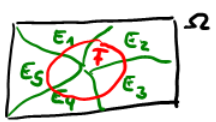
\includegraphics[scale=0.25]{./pic/SatzTotalerWahrscheinlichkeit.png}
  	\subsection{Vierfeldertafel}
  	$ P(F) = P(F \cap E ) + P(F \cap \overline{E}) $\\
  	$ P(\overline {F}) = P(\overline{F} \cap E) + P(\overline{F} \cap E) $\\
  	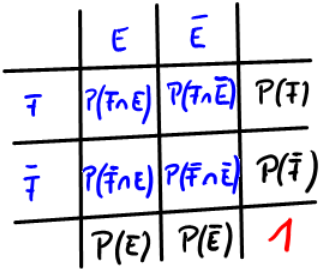
\includegraphics[scale=0.25]{./pic/Vierfeldertafel}
  	\textbf{Satz 2.2 oben: }
  	$ P(E \cap F)  =  P(E) \cdot P(F|E) = P(F) \cdot P(E|F) $
  	\textbf{Tafel}
  	$ = P(F) - P(F \cap \overline{E}) $
  	$ = P(E) - P(\overline{F} \cap E) $; 
  $ P(\overline{F} | E) = 1 - P(F | E) $
  \subsection{Formel von Bayes}
  Hilfreich, wenn man man $P( F | E_{i} )$ kennt, aber nicht $P(E_{k}|F)$
  \textbf{Satz 2.4}
  $P(E_{k} | F) = \frac{ P(F | E_{k}) \cdot P(E_{k})}{ \underbrace{\sum_{i=1}^{n}P(F|E_{i}) \cdot P(E_{i})}}$\\
\textbf{Nur Nenner!}P(F) aus dem Satz der totalen Wahrscheinlichkeit.
  \subsection{Stochastische Unabhängigkeit}
  \textbf{Übung}
  Die Ereignisse E und F heißen (stochastisch) unabhängig, wenn die Information über das Eintreten des einen Ereignisses die Wahrscheinlichkeit für das Eintreten des anderen Ereignisses nicht ändert, d.h. falls\\
  $\underbrace{P(E|F)}= P(E)  \text{ or }   P(E\cap F) = P(E) \cdot P(F)$\\
  $= \frac{P(E \cap F)}{P(F)}$\\
  \textbf{Es gilt}
  Falls die Ereignisse E, F unabhängig sind, dann sind auch: 
  $\circ  E, \overline{F}$;  
  $\circ  \overline{E} , F$;  
  $\circ \overline{E}, \overline{F}$ unabhängig\\
  \textbf{Bemerkung}\\
  	$ \circ $ Stochastische Unabhängigkeit bedeutet nicht notwendigerweise eine kausale Abhängigkeit; 
  	$ \circ $ Veranschaulichung mit Venn Diagramm
  	  \includegraphics[scale=0.23]{./pic/StochastischeUnabhängigkeit.png}
  	  \includegraphics[scale=0.23]{./pic/StochastischeAbhängigkeit.png}\\
  	$\circ$ $A, B \ne \varnothing$ und $A \cap B  = \varnothing$\\
  	$P(A\cap B) \stackrel{?}{=} P(A) \cdot P(B)$\\
  	$ \varnothing \ne P(A) \cdot P(B)$ da P(A) > 0 und P(B)> 0\\
  	=> A, B stochastisch abhängig
%\input{inhalt/aussagen}
%\input{inhalt/mengen}
%\input{inhalt/relationen}
%\input{inhalt/abbildungen}
%\input{inhalt/beweise} 
%\input{inhalt/graphen}
%\input{inhalt/graphalgo}
%\input{inhalt/bool}
%\input{inhalt/formeln}
\end{multicols*}
\end{document}